\documentclass{article}[18pt]
\usepackage[utf8]{inputenc}
\usepackage[margin=0.7in]{geometry}
\usepackage{amsmath}
\usepackage{titlesec}
\usepackage{pgfplots}
\usepackage{graphicx}
\usepackage[english]{babel}
\usepackage{fancyhdr}
\usetikzlibrary{decorations, decorations.text,positioning,quotes,arrows.meta,decorations.markings,3d,shapes,decorations.pathmorphing}
\pgfplotsset{width=10cm,compat=1.9}

\titlespacing\section{0pt}{14pt plus 4pt minus 2pt}{0pt plus 2pt minus 2pt}
\newlength\tindent
\setlength{\tindent}{\parindent}
\setlength{\parindent}{0pt}
\renewcommand{\indent}{\hspace*{\tindent}}

\pagestyle{fancy}
\fancyhf{}
\rhead{Sam Robbins 13SE}
\lhead{A Level Physics - Fields}
\rfoot{Page \thepage}


\tikzstyle{arrow} = [thick,->,>=stealth]



\begin{document}
\begin{center}
\underline{\huge Electromagnetic Induction}
\end{center}
\section{Generating Electricity}
$ $\\
$ $\\

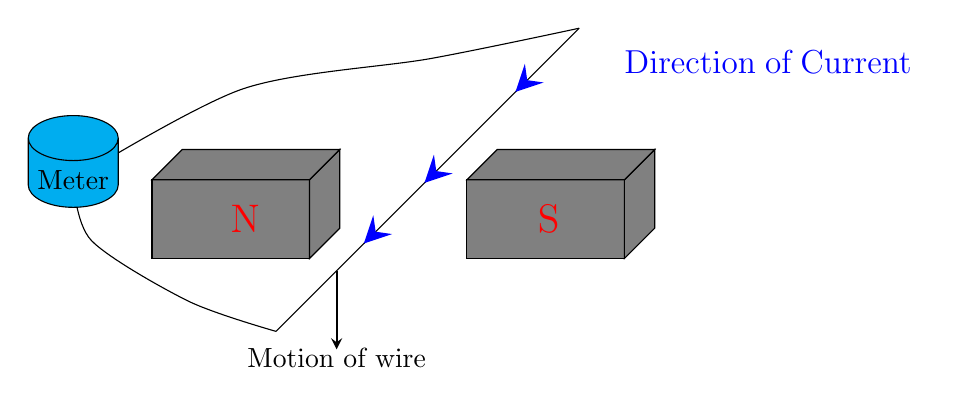
\begin{tikzpicture}
\tikzset{myptr/.style={decoration={markings,mark=at position 1 with %
    {\arrow[scale=3,>=stealth,blue]{>}}},postaction={decorate}}}
\pgfmathsetmacro{\cubex}{2}
\pgfmathsetmacro{\cubey}{1}
\pgfmathsetmacro{\cubez}{1}
\draw[black,fill=gray] (0,0,0) -- ++(-\cubex,0,0) -- ++(0,-\cubey,0) -- ++(\cubex,0,0) -- cycle;
\draw[black,fill=gray] (0,0,0) -- ++(0,0,-\cubez) -- ++(0,-\cubey,0) -- ++(0,0,\cubez) -- cycle;
\draw[black,fill=gray] (0,0,0) -- ++(-\cubex,0,0) -- ++(0,0,-\cubez) -- ++(\cubex,0,0) -- cycle;

\draw[black,fill=gray] (4,0,0) -- ++(-\cubex,0,0) -- ++(0,-\cubey,0) -- ++(\cubex,0,0) -- cycle;
\draw[black,fill=gray] (4,0,0) -- ++(0,0,-\cubez) -- ++(0,-\cubey,0) -- ++(0,0,\cubez) -- cycle;
\draw[black,fill=gray] (4,0,0) -- ++(-\cubex,0,0) -- ++(0,0,-\cubez) -- ++(\cubex,0,0) -- cycle;


\coordinate  (d5) at (1.5,0,5){};
\coordinate  (d6) at (1.5,0,-5){};

\draw []       (d5)--(d6);
\node[text width=4cm,red] at (1,-0.5) {\Large{N}};
\node[text width=4cm,red] at (4.9,-0.5) {\Large{S}};
\draw [arrow] (1.5,0,3) -- node[anchor=west,below,yshift=-10] {Motion of wire} (1.5,-1,3);
\draw [myptr] (1.5,0,-3) -- (1.5,0,-2.9);
\draw [myptr] (1.5,0,0) -- (1.5,0,0.1);
\draw [myptr] (1.5,0,2) -- (1.5,0,2.1);
\node[text width=4cm,blue] at (6,1.5) {\large{Direction of Current}};
\draw [black] plot [smooth] coordinates { (1.5,0,5) (0,0,4) (-2,0,2) (-3,0,0)};
\draw [black] plot [smooth] coordinates { (1.5,0,-5) (0,0,-4) (-2,0,-3) (-3,0,0)};
\node[cylinder, draw, shape aspect=.5,shape border rotate=90,fill=cyan] at (-3,0) {Meter};
\end{tikzpicture}\\
When a conductor is moved through a magnetic field an emf is \textbf{induced} across the ends of the conductor\\
\\
The emf will be greater when:
\begin{itemize}
\item The conductor is moved more quickly
\item The magnetic field is stronger
\item There is a longer length of conductor in the magnetic field
\end{itemize}
No emf will be induced if the conductor is parallel to the field lines\\
\\
A current will flow if the conductor is part of a complete circuit
\subsection{Explaining electromagnetic induction}
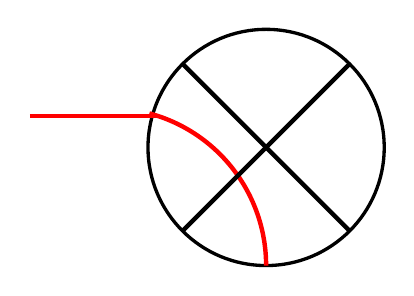
\begin{tikzpicture}
\filldraw[color=black,fill=none,very thick](-1,0) circle (1.5);
\draw[ultra thick, -,red] (-1,-1.5) arc (0:75:2);
\draw[ultra thick, red] (-4,0.4) -- (-2.4,0.4);
\draw[ultra thick, black] (0.06,1.06) -- (-2.06,-1.06);
\draw[ultra thick, black] (-2.06,1.06) -- (0.06,-1.06);

\end{tikzpicture}\\
\\
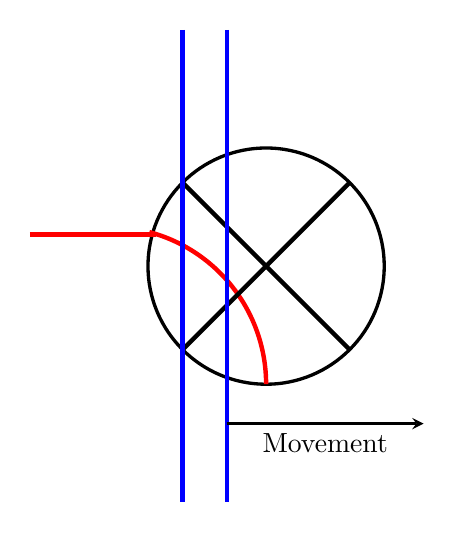
\begin{tikzpicture}
\tikzstyle{arrow} = [thick,->,>=stealth]
\filldraw[color=black,fill=none,very thick](-1,0) circle (1.5);
\draw[ultra thick, -,red] (-1,-1.5) arc (0:75:2);
\draw[ultra thick, red] (-4,0.4) -- (-2.4,0.4);
\draw[ultra thick, black] (0.06,1.06) -- (-2.06,-1.06);
\draw[ultra thick, black] (-2.06,1.06) -- (0.06,-1.06);


\draw[ultra thick, blue] (-2.06,3) -- (-2.06,-3);
\draw[ultra thick, blue] (-1.5,3) -- (-1.5,-3);

\draw [arrow] (-1.5,-2) -- node[anchor=north] {Movement} (1,-2);
\end{tikzpicture}
\newpage
\section{The laws of electromagnetic induction}
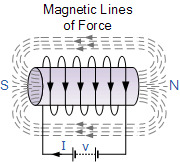
\includegraphics[width=5cm]{magnetic_induction.jpg}\\
North Pole - Anticlockwise current flow\\
South Pole - Clockwise current flow\\
\section{Lenz's law}
The direction of the induced emf is always such as to oppose the change that is causing it.\\
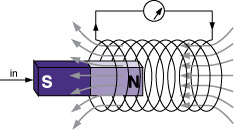
\includegraphics[width=5cm]{lenz.jpg}\\
As the magnet is pushed into the coil it induces an emf in the coil, this produces a magnetic field which opposes the potion. When removing the magnet the polarity will be inversed.\\
\section{Faraday's law}
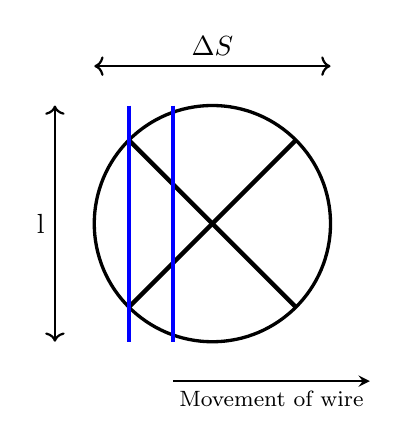
\begin{tikzpicture}
\tikzstyle{arrow} = [thick,->,>=stealth]
\filldraw[color=black,fill=none,very thick](-1,0) circle (1.5);

\draw[ultra thick, black] (0.06,1.06) -- (-2.06,-1.06);
\draw[ultra thick, black] (-2.06,1.06) -- (0.06,-1.06);


\draw[ultra thick, blue] (-2.06,1.5) -- (-2.06,-1.5);
\draw[ultra thick, blue] (-1.5,1.5) -- (-1.5,-1.5);

\draw [arrow] (-1.5,-2) -- node[anchor=north] {\footnotesize{Movement of wire}} (1,-2);
\draw[thick, <->] (-3,-1.5) -- (-3,1.5) node[anchor=east,midway] {l};

\draw[thick, <->] (-2.5,2) -- (0.5,2) node[anchor=south,midway] {$\Delta S$};
\end{tikzpicture}\\
\\
\begin{tabular}{r l}
Work done&$=F\times S$\\
&$=BIl\times\Delta S$
\end{tabular}\\
\\
Charge transfer, $Q=I\times\Delta t$\\
\\
$\epsilon=\dfrac{\text{Work done}}{\text{Charge}}=\dfrac{BIl\times\Delta S}{I\times\Delta t}=\dfrac{BA}{\Delta t}$\\
\\
\textcolor{red}{B=Magnetic flux density=$\dfrac{\phi}{A}$}\\
\textcolor{red}{$\phi$ = Magnetic flux}
$$\epsilon=\dfrac{\phi}{\Delta t}$$
\newpage
Faraday's law of electromagnetic induction is equal to the rate of change of flux(linkage) through the circuit.\\
\\
Flux linkage refers to coils, $N\phi$ replaces $\phi$ where N is the number of coils.
$$\epsilon=-N\dfrac{\Delta\phi}{\Delta t}$$
This equation may need to be expanded depending on the example
\subsection{Example}
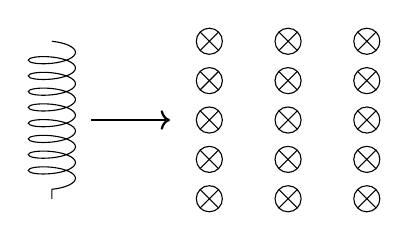
\begin{tikzpicture}[cross/.style={path picture={ 
  \draw[black]
(path picture bounding box.south east) -- (path picture bounding box.north west) (path picture bounding box.south west) -- (path picture bounding box.north east);
}},decoration={coil}]

 \node [draw,circle,cross,minimum width=2 mm] at (2,0){}; 
 \node [draw,circle,cross,minimum width=2 mm] at (2,-0.5){};
 \node [draw,circle,cross,minimum width=2 mm] at (2,-1){};
 \node [draw,circle,cross,minimum width=2 mm] at (2,-1.5){};
 \node [draw,circle,cross,minimum width=2 mm] at (2,-2){};
 
  \node [draw,circle,cross,minimum width=2 mm] at (3,0){}; 
 \node [draw,circle,cross,minimum width=2 mm] at (3,-0.5){};
 \node [draw,circle,cross,minimum width=2 mm] at (3,-1){};
 \node [draw,circle,cross,minimum width=2 mm] at (3,-1.5){};
 \node [draw,circle,cross,minimum width=2 mm] at (3,-2){};
 
   \node [draw,circle,cross,minimum width=2 mm] at (4,0){}; 
 \node [draw,circle,cross,minimum width=2 mm] at (4,-0.5){};
 \node [draw,circle,cross,minimum width=2 mm] at (4,-1){};
 \node [draw,circle,cross,minimum width=2 mm] at (4,-1.5){};
 \node [draw,circle,cross,minimum width=2 mm] at (4,-2){};
 
 \draw[decorate, decoration={aspect=0.3, segment length=2mm, amplitude=3mm}] (0,0) --(0,-2);
 
 \draw[thick, ->] (0.5,-1) -- (1.5,-1) ;
\end{tikzpicture}\\
\\
\textcolor{red}{$\epsilon=-N\dfrac{B\Delta A}{\Delta t}$}




\end{document}